\documentclass[11pt]{article} 
\usepackage[utf8]{inputenc}

%%% PAGE DIMENSIONS
\usepackage{geometry}
\geometry{a4paper}

\usepackage{graphicx} % support the \includegraphics command and options

% \usepackage[parfill]{parskip} % Activate to begin paragraphs with an empty line rather than an indent

%%% PACKAGES
\usepackage{float}
\usepackage{booktabs}
\usepackage{array}
\usepackage{paralist}
\usepackage{verbatim}
\usepackage{subfig} 
\usepackage{fancyhdr}
\usepackage{amsmath}


\pagestyle{fancy} % options: empty , plain , fancy
\renewcommand{\headrulewidth}{0pt} % customise the layout...
\lhead{}\chead{}\rhead{}
\lfoot{}\cfoot{\thepage}\rfoot{}

\usepackage{sectsty}
\allsectionsfont{\sffamily\mdseries\upshape}

\usepackage{listings}
\usepackage{color}

\definecolor{mygreen}{rgb}{0,0.6,0}
\definecolor{mygray}{rgb}{0.5,0.5,0.5}
\definecolor{mymauve}{rgb}{0.58,0,0.82}

\lstset{ 
  backgroundcolor=\color{white},   % choose the background color; you must add \usepackage{color} or \usepackage{xcolor}; should come as last argument
  basicstyle=\footnotesize,        % the size of the fonts that are used for the code
  breakatwhitespace=false,         % sets if automatic breaks should only happen at whitespace
  breaklines=true,                 % sets automatic line breaking
  captionpos=b,                    % sets the caption-position to bottom
  commentstyle=\color{mygreen},    % comment style
  firstnumber=1000,                % start line enumeration with line 1000
  frame=single,	                   % adds a frame around the code
  keepspaces=true,                 % keeps spaces in text, useful for keeping indentation of code (possibly needs columns=flexible)
  keywordstyle=\color{blue},       % keyword style
  language=Python,                 % the language of the code
  numbers=left,                    % where to put the line-numbers; possible values are (none, left, right)
  numbersep=5pt,                   % how far the line-numbers are from the code
  numberstyle=\tiny\color{mygray}, % the style that is used for the line-numbers
  rulecolor=\color{black},         % if not set, the frame-color may be changed on line-breaks within not-black text (e.g. comments (green here))
  showspaces=false,                % show spaces everywhere adding particular underscores; it overrides 'showstringspaces'
  showstringspaces=false,          % underline spaces within strings only
  showtabs=true,                   % show tabs within strings adding particular underscores
  stepnumber=1,                    % the step between two line-numbers. If it's 1, each line will be numbered
  stringstyle=\color{mymauve},     % string literal style
  tabsize=2,	                   % sets default tabsize to 2 spaces
  title=\lstname                   % show the filename of files included with \lstinputlisting; also try caption instead of title
}


\title{Práctica 1: Regresión Lineal}
\author{Ana Martín Sánchez, Nicolás Pastore Burgos}
\date{21/09/2021} 

\begin{document}
\maketitle

\section{Descripción de la práctica}

 En esta práctica, se pedía aplicar el método de regresión logística sobre dos conjuntos de datos. 
 
 En primer lugar, se nos da un conjunto de datos que relaciona dos variables: la nota de varios candidatos en un examen de acceso a la universidad, y si fueron admitidos o no.
 Después, se nos presenta un conjunto de datos que relaciona el resultado de someter a varios microchips a dos controles de calidad, y si los superan o no.

Para el primer conjunto de datos, se puede observar que los datos se pueden separar linealmente, definiendo una barrera entre los que superan los exámenes de acceso y los que no. En el segundo caso, esta barrera no es lineal.

Por ello, en el primer caso podemos aplicar la regresión logística sin problemas pero, en el segundo conjunto de datos, tendremos que utilizar la versión regularizada de este mismo algoritmo.


\newpage
\section{Solución propuesta}

\subsection{Resultados obtenidos}

\subsubsection {Parte 1}

Conseguimos implementar una función que devuelve un coste óptimo de 0.203 para los datos proporcionados, y que permite dibujar una recta como se muestra en la figura 1.

 \begin{figure}[h!]
    \begin{center}
    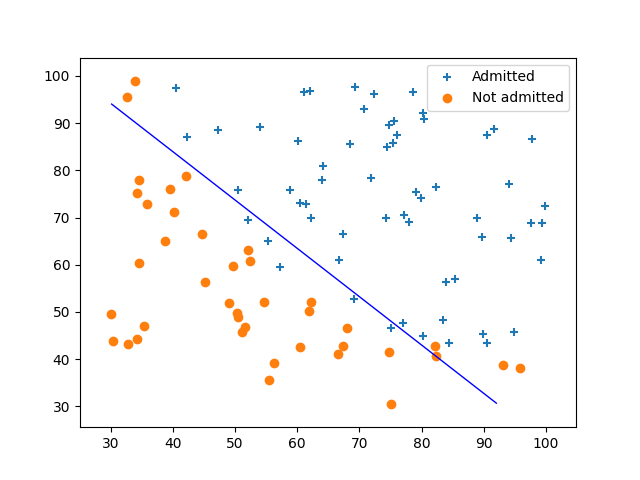
\includegraphics[width=\textwidth]{Imagenes/Recta.png}
    \caption{Gráfica que muestra la recta calculada para los datos proporcionados por el enunciado.}
    \label{fig:Gráfica que muestra la recta calculada para los datos proporcionados por el enunciado.}
    \end{center}
 \end{figure}

\subsubsection {Parte 2}

En esta parte hemos conseguido los reultados esperados; hemos podido implementar una función de coste y otra de descenso de gradiente tales que, para
 \begin{equation*}
    \theta = 0
  \end{equation*}
 \begin{equation*}
    \lambda = 1
  \end{equation*}
el coste inicial es de 0.693, y permite dibujar una barrera como la que se muestra en la figura 2.

También es interesante remarcar que, cambiando el valor de lambda, se regulariza el descenso, pero se sigue consiguiendo un resultado correcto.

 \begin{figure}[h!]
    \begin{center}
    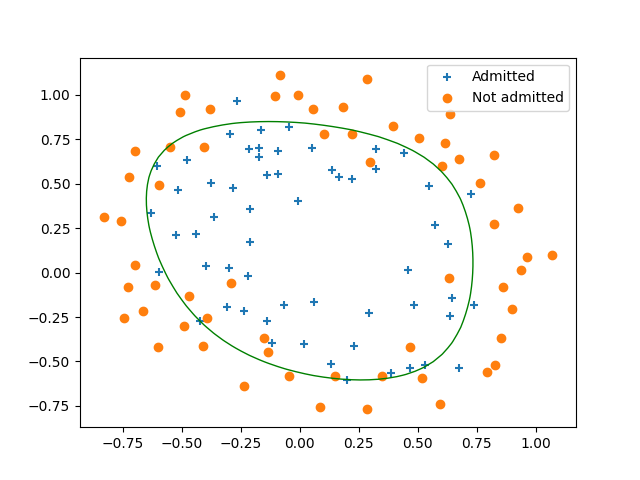
\includegraphics[width=\textwidth]{Imagenes/Circulico.png}
    \caption{Gráfica que muestra la barrera que separa los microchips que pasan los tests de los que no.}
    \label{fig:Resultados}
    \end{center}
 \end{figure}

\newpage
\subsection{Implementación}

\lstinputlisting[language=Python]{main.py}


\end{document}
